%%%%%%%%%%%%%%%%%%%%%%%%%%%%%%%%%%%%%%%%%%%%%%%%%%%%%%%%%%%%%%%%%%%%%%%%
%                                                                      %
%     File: Thesis_Implementation.tex                                  %
%     Tex Master: Thesis.tex                                           %
%                                                                      %
%     Author: João D. Lopes                                            %
%     Last modified :  31 May 2016                                     %
%                                                                      %
%%%%%%%%%%%%%%%%%%%%%%%%%%%%%%%%%%%%%%%%%%%%%%%%%%%%%%%%%%%%%%%%%%%%%%%%

\chapter{Architecture}
\label{chapter:architecture}

Versat is designed to do signal processing, so its architecture has a
Data Engine (DE) unit that performs data computation. Since Functional
Units (FUs) are fully connected, that means there is more than one way
to make a datapath. This feature has been implemented with the objective
of simplifying the compiler technology, which can be very complex. A
configuration module holds the configuration of the DE, i.e., it
specifies the current datapath, and can also temporarily store tens of
other configurations, which can be switched at runtime. The Versat
top-level entity is represented in figure~\ref{fig_top}.

\begin{figure}[!htb]
\centering
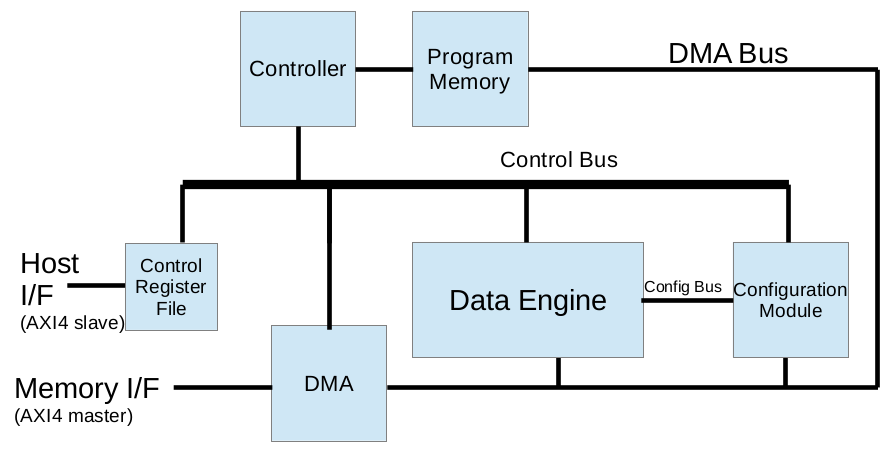
\includegraphics[width=.7\textwidth]{drawings/top}
\caption{Versat top-level entity}
\label{fig_top}
\end{figure}

In order to have less dependency from the host CPU, it has been
decided that Versat should have a simple controller. This way, it can
do self-reconfiguration without engaging the host, which becomes free
for other more useful tasks. The controller is programmable and has an
instruction memory where Versat programs or kernels are stored.
To communicate with the host processor, Versat has the Control
Register File (CRF), which is shared with the host.

The controller can write partial configurations to the configuration
module, command the configuration module to save a configuration or to
restore a saved configuration.

Versat as two interfaces that can be selected at compile time: a
Serial Peripheral Interface (SPI) and a parallel bus interface. The
SPI interface is used when an off-chip device is the host. Versat is a
slave SPI device and the host is a master SPI device. The parallel bus
interface is used when the host is some embedded processor. This bus
had a generic format which has been recently replaced with the
Advanced Extensible Interface - AXI4. It is an interface designed by
ARM, which derives from the Advanced Microcontroller Bus Architecture
(AMBA). Associated with the parallel interface is a DMA module used
for data transfers from/to an external memory.


%%%%%%%%%%%%%%%%%%%%%%%%%%%%%%%%%%%%%%%%%%%%%%%%%%%%%%%%%%%%%%%%%%%%%%%%
\section{Data Engine}
\label{section:dataEngine}

The Data Engine (DE) is designed to do vector computations. To
accomplish this goal, instead of regular registers, it has 4 Random
Access Memories (RAMs - with the size of 2048 words of 32 bits),
which work as vector registers.

It also contains several FUs that actually perform data computation: 2
ALUs, 4 smaller ALUs (AluLite), 4 multipliers and 1 barrel shifter. The FUs are
connected to each other by a large bus, formed by the output of every
FU -- the data bus. Each FU input can then select a section of this
bus by using multiplexers (MUXs). A simple diagram in
figure~\ref{fig_de} illustrates the DE.

\begin{figure}[!htb]
\centering
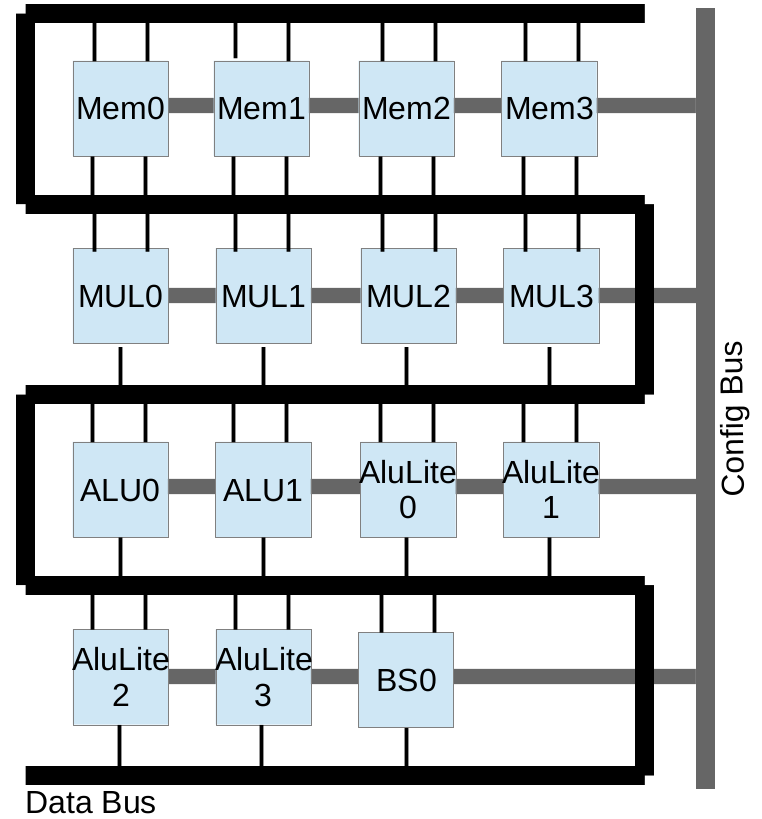
\includegraphics[width=.5\textwidth]{drawings/de}
\caption{Data engine}
\label{fig_de}
\end{figure}

The data bus, in addition to the output from the FUs, has 2 additional
values: the constants 0 and 1, which are commonly used in many
datapaths, so there is no need to store these constants. Another bus
is used to configure the DE to create datapaths: the configuration
bus.

An ALU can do any of the following operations:
\begin{itemize}
	\item logical OR;
	\item logical AND;
	\item logical AND with one of the operands negated;
	\item logical XOR;
	\item addition;
	\item subtraction;
	\item sign extension of 8 bits;
	\item sign extension of 16 bits;
	\item arithmetic right shift;
	\item logic right shift;
	\item unsigned comparison;
	\item signed comparison;
	\item counting leading zeros;
	\item maximum;
	\item minimum;
	\item absolute value.
\end{itemize}

The AluLite units can perform only the first six operations. This way,
the AluLite units are smaller and more power efficient. Both ALU types
have 2 clock cycles of latency.

The multiplier produces a 64-bit result from two 32-bit operands and
has two configuration parameters. One parameter allows selecting the
lower or higher 32 bits of the result. The other parameter forces the
multiply result to be left-shifted by 1 bit. This configuration is
useful when operands are in the common Q1.31 fixed-point
format. Setting the first parameter to select the high part of the
result and the second parameter to shift left by 1, allows the
multiplication of two Q1.31 operands to yield Q1.31 result.  This unit
has 3 clock cycles latency.

The barrel shifter can perform left shifts and logic and arithmetic
right shifts. The number of bits to shift is one operand and the value
to be shifted is the other operand. This FU has only 1 clock cycle
of latency.

All FUs have the possibility to store some value in their output
register to be used in the datapath. To do that it is required that
the FU is configured as disabled. This is useful in case the
computation datapath has one or more constants.

The DE memories are dual-port RAMs and each port has attached an
address generator. The address generator is the block that allows
Versat to execute two nested loops with just one configuration, with
the restriction that the inner loop has a maximum of 32 iterations and
the outer loop has a maximum of 2048 iterations.

%%%%%%%%%%%%%%%%%%%%%%%%%%%%%%%%%%%%%%%%%%%%%%%%%%%%%%%%%%%%%%%%%%%%%%%%
\section{Configuration Module}
\label{section:configuration}

The configuration module is composed by a configuration register,
where the next configuration is set, and the configuration memory,
where some configurations are stored to be used later, as it is visible in
figure~\ref{fig_conf}.

The configuration register is a register of 660 bits, fully
addressable, which means that it is possible to change only one field
of this register. This feature takes advantage that in most
applications there is a high likelihood that one configuration will be
reused again in a nearby instant of time (time locality). Therefore,
it is possible to do partial reconfiguration in a few clock cycles.

The configuration module also has a shadow configuration
register. This register holds the configuration that the DE is
executing, so another one can be generated in parallel with the DE
execution.

\begin{figure}[!htb]
\centering
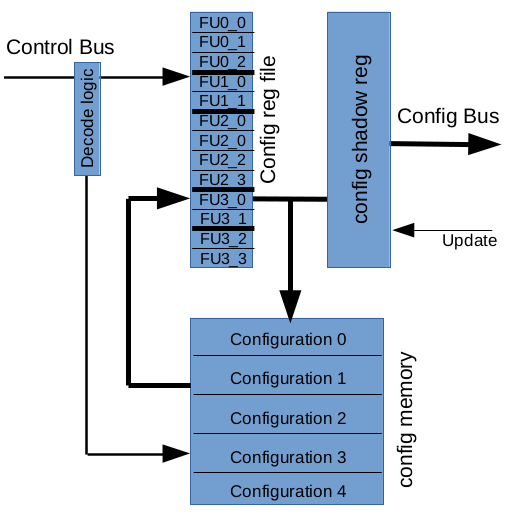
\includegraphics[width=.55\textwidth]{drawings/conf}
\caption{Configuration Module}
\label{fig_conf}
\end{figure}

The configuration memory has 64 positions, used to keep some
configurations previously generated to reuse them later. This memory
is a dual-port memory. One port has 660 bits (configuration width),
which means that configurations can be loaded/stored from/to the
configuration register in just 1 clock cycle. The other is a 32-bit
port used to load and store configurations in the external memory
through the DMA. This second port can expand the configuration memory
beyond 64 configurations. This scheme is designed so that one can
study the difference between working with pre-built configurations
stored in external memory and generating configurations using the
Versat controller.

%%%%%%%%%%%%%%%%%%%%%%%%%%%%%%%%%%%%%%%%%%%%%%%%%%%%%%%%%%%%%%%%%%%%%%%%
\section{Controller}
\label{section:controller}

The Versat controller has a minimal architecture
(Fig.~\ref{fig_control}) to support reconfiguration, data movement and
host interaction. It contains 3 main registers: the program counter
(register PC), the accumulator (register A) and the data pointer
(register B). The instruction whose address is pointed by the PC is
decoded so that an opcode and an immediate value (often a memory
address) are extracted from it.

\begin{figure}[!htb]
\centering
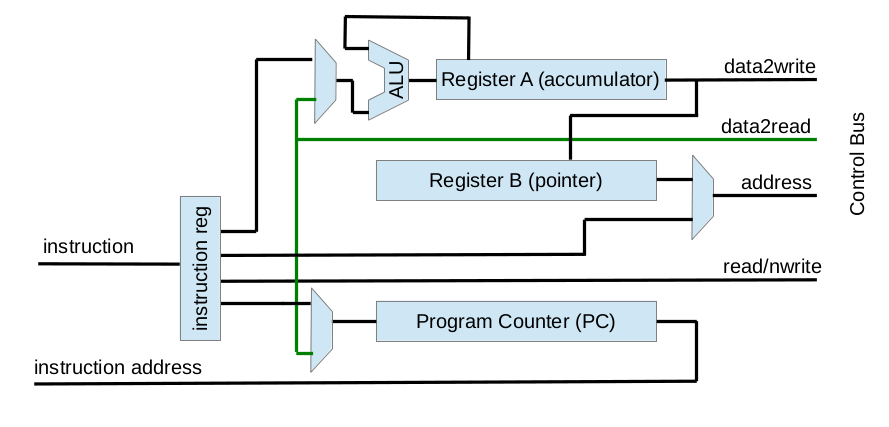
\includegraphics[width=.8\textwidth]{drawings/control}
\caption{Controller}
\label{fig_control}
\end{figure}

Register A is the destination of all operations that the controller
performs, and is also often one of the operands (accumulator
architecture).

On the other hand, register B, which is addressable by the controller,
is used to implement indirect loads and stores. Its contents is the
load/store address.

The controller has an instruction set of only 16 instructions (opcode
of 4 bits, immediate value of 16 bits). These allow the controller to
perform the following actions: loads/stores to/from the accumulator,
arithmetic and logic operations and branches. There are three types of
load instructions: of immediate constants, direct (from an immediate
address) and from an indirect address stored in register B. The stores
can be direct or indirect.

In order to increase frequency, by reducing the critical path, the
controller takes 2 clock cycles to fetch one instruction, in
pipeline. For simplicity, it executes every instruction that is
fetched. In other words, it has 2 delay slots in case of a branch
instruction. These delay slots can be filled with a no-operation
instruction (NOP), but the compiler/programmer can also use them to
execute useful instructions. For instance, in the case of a {\tt for}
loop, the delay slots can be used to write the iteration count to some
register.

The controller can handle host procedure calls. For each procedure it
is necessary to read parameters from the control register file and
configure and execute the DMA and DE multiple times. DMA and DE
threads can be spawned, hiding part of the controller execution time,
as will be shown later.


%%%%%%%%%%%%%%%%%%%%%%%%%%%%%%%%%%%%%%%%%%%%%%%%%%%%%%%%%%%%%%%%%%%%%%%%
\section{DMA}
\label{section:dma}

One of the crucial factors to guarantee acceleration is the rapidity
at which data is moved in and out of Versat. Accessing data words one
by one in the external memory is out of the question. Data must be
moved in blocks to amortize the memory latency that is always present
when an external memory device has to be used.

The DMA engine is operated by the Versat controller to transfer a data
burst from external memory to one of the Versat's data engine
memories, or from one of Versat's data engine memories to the external
memory. It also possible to move data to the instruction memory or
to/from the configuration memory.

From the Versat controller point of view the DMA is memory mapped and
the following DMA registers can be accessed: the external address
register, the internal address register, the size register, the
direction register and the status register. The external address
register holds the transfer start address in the external memory (32
bits), and the internal address register holds the transfer starts
address in Versat (14 bits). The size register has the number of words
to be transferred (8 bits to support transactions of up to 256 words,
which is the maximum for AXI4). The direction register tells the DMA
state machine if it is a transfer form Versat to the external memory
or vice-versa. When this register is written with a value different
from zero the transfer starts. At the end of the transfer it self
clears. The status register tells the controller whether the DMA is
busy or ready to initiate a new transaction; it also informs if an
error has occurred.

%%%%%%%%%%%%%%%%%%%%%%%%%%%%%%%%%%%%%%%%%%%%%%%%%%%%%%%%%%%%%%%%%%%%%%%%
\section{Program memory}
\label{section:programMemory}

The program memory is divided in two parts: the boot ROM (256 words of
32 bits) and the instruction memory RAM (2048 words of 32
bits). However, it is addressable as a single memory with the value
stored in the PC register. The first 256 addresses are used to address
the boot ROM, the others to address the instruction memory.

The boot ROM holds the instructions that allow Versat to communicate
with the host processor. Basically is is used for the host to call
Versat kernels and to load/store values in any addressable memory
position within Versat.

The instruction memory, that needs to be loaded, contains the
instructions related with the kernel. This memory can not be read
(except to execute instructuions) but it can be written to load the
kernel instructions.

%%%%%%%%%%%%%%%%%%%%%%%%%%%%%%%%%%%%%%%%%%%%%%%%%%%%%%%%%%%%%%%%%%%%%%%%
\section{Control Register File}
\label{section:controlRegisterFile}

The CRF has 16 registers of 32 bits each, and is implemented with a
dual-port register file (one port for the host and the other port for
Versat). These registers are used to establish the communication
between the two processors. To perform that, both can read and write
to the CRF.


\begin{comment}
After hardware reset the Versat, through boot ROM program, waits a
host command. Three registers of the CRF are used for this purpose:
one as a command register (R14), two as an address register (R0) and
another one as a data register (R15).

There are 3 commands (for now): read command, that allow the host to
access some data from Versat (for debug, for instance), write command,
that host uses to write some data into Versat, and run command, that
indicates to Versat to run some kernel.

In case of read, the host writes the read command into R14 (\#4), the
base address into R0 and waits that Versat write Acknowledge (Ack -
\#3) into R14. When it does, he read data from R15, clean Ack value
from R14 and waits for a new Ack. On Versat side, which is reading R0
until it has a nonzero value, after host command (written on R0), he
process the command given and get into a certain loop according the
command. In this case, after he loads the R0 value into RB, get into a
loop that reads R14 until it has a value that is not Ack. When this
happens, he checks if R14 value is equal to finish (\#2). If it is, go
back to boot ROM base address (cleans the R0 and wait it has a nonzero
value again), if not, read from the address pointed by RB, put the
data into R15, increment RB, write the Ack into R14 and go back to
read R14 loop (waits that R14 has a different value again).

In case of write, the host writes the first data value into R15, the
command into R14 and the base address into R0 (there is no write
command, it just have to be a different value that other commands uses
on protocol - i.e. \#0). When it does, he get into a loop that reads
R14 and wait for Ack. On Versat side, after processing the command
given, loads the R0 value into RB and get into a loop that reads R14
until it has a value that is not Ack. When this happens, he checks if
R14 value is equal to finish (\#2). If it is, go back to boot ROM base
address (cleans the R0 and wait it has a nonzero again), if not, write
R15 value into the address pointed by RB, increment RB, write the Ack
into R14 and go back to read R14 loop (waits that R14 has a different
value again).

For the execution of a kernel, the CRF is used by the host also to
pass parameters to Versat and by Versat to return status information
to the host (the registers used to do that are undefined, depends on
the kernel it self). After a host command, Versat do an unconditional
branch to address written on R0, starting the kernel execution.
\end{comment}
